\subsubsection*{Problem definition}

To verify the linear elastic transverse isotropic material model in the three dimensional case, the tensile test analyzed in Sec.~\ref{subsec:transiso_tens2d} was simulated using a rectangular sample with an edge length $l=10\,$mm and a height $h=1\,$mm. According to the twodimensional case, a vertically arranged laminated material structure is assumed. The direction of anisotropy, which is defined by a vector $\miu{a}{}{}$ is perpendicularly oriented to the material layers. During simulation, the direction of anisotropy is rotated counterclockwise in the $xy$-plane from $\varphi=0^{\circ}$ to $\varphi=180^{\circ}$. 

Within the context of the different opportunities offered by the input structure of {\sl OpenGeoSys} to define the anisotropy direction, the coefficients of the unit normal vector which is parallel to the direction of anisotropy are given as $n_x=\cos\varphi$, $n_y=\sin\varphi$, and $n_z=0$. Considering the case that the basis vectors of the local Cartesian coordinate system for transverse isotropic materials are provided by consecutive rotations of the plane of isotropy about the global $y$($x_2$)-axis and the $\bar{x}$($\bar{x}_1$)-axis of the once rotated system, the angle $\alpha$ has a constant value of $90^{\circ}$, whereas the angle $\beta$ changes from $0^{\circ}$ to $-180^{\circ}$. Using the angles known from applications in structural geology to generate the constitutive rotation matrices, the dip $\phi$ has the constant value of $90^{\circ}$, and the azimuth varies from $90^{\circ}$\dots$0^{\circ}$ (for $0^{\circ}\leq\varphi\leq 90^{\circ}$) and $360^{\circ}$\dots$270^{\circ}$ (for $90^{\circ}\leq\varphi\leq 180^{\circ}$) respectively.

For details of the model (geometry, boundary conditions, material orientation) see Fig.~\ref{tens_transiso_model_3d}.

\begin{figure}[!htb]
\begin{center}
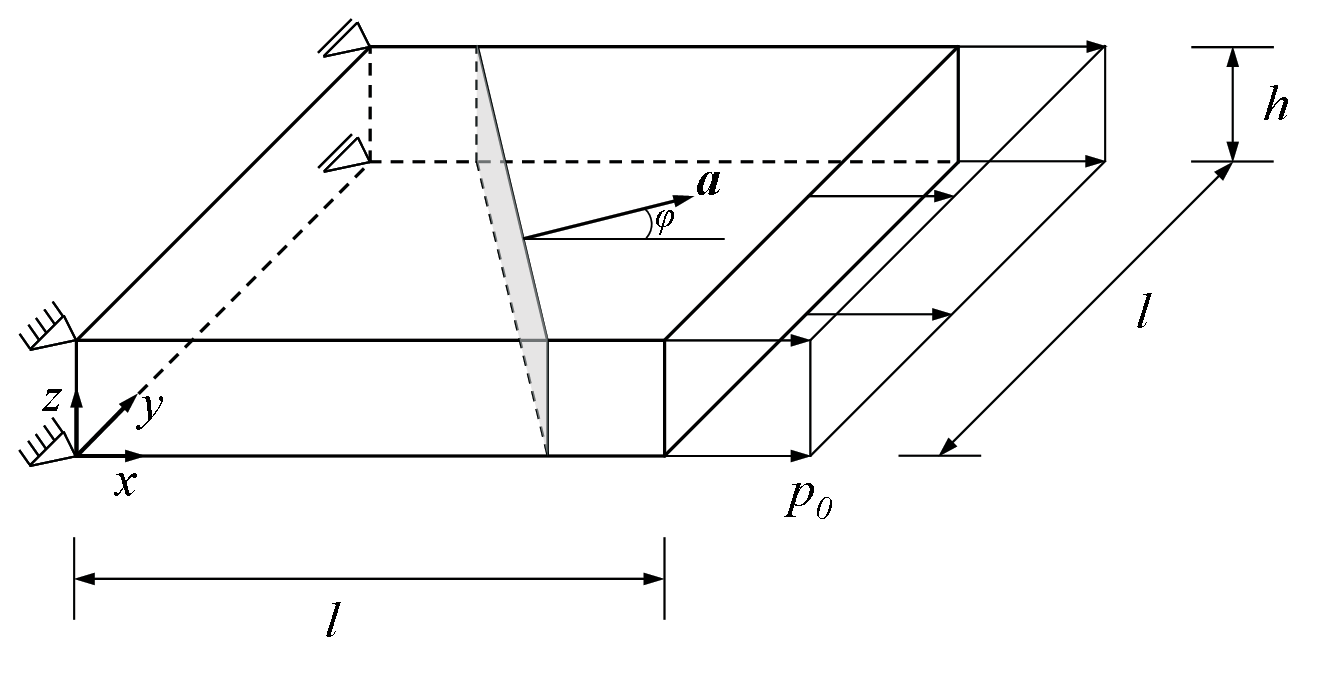
\includegraphics[width=0.7\textwidth]{M/figure/tenstest_model_3D.eps}
\end{center}
\caption{Tensile test. Threedimensional model definition according to Fiolka \cite{Fiolka:2007}. Vector $\miu{a}{}{}$ defines the direction of anisotropy.} 
\label{tens_transiso_model_3d}
\end{figure}

\subsubsection*{Initial and boundary conditions}

The initial and boundary conditions are the same as described for the two dimensional example  (cf. Sec.~\ref{subsec:transiso_tens2d}). The plane strain condition assumed for the twodimensional case was realized preventing any displacement in $z$-direction on the upper and lower boundary surfaces of the sample.

\subsubsection*{Material properties}

The material parameters are given in Tab.~\ref{matpar_transiso_tens}, as in the twodimensional case (cf. Sec.~\ref{subsec:transiso_tens2d}).

\subsubsection*{Results}

The results in the corresponding corner nodes of the sample are exactly the same as presented in Fig.~\ref{tens_transiso_test_2d} (cf. Sec.~\ref{subsec:transiso_tens2d}).

\subsubsection*{Benchmark deposit}

\begin{tabular}{|l|l|l|}
  \hline
  Benchmark & Problem type & Path in benchmark deposit \\
  \hline
 \emph{m\_e\_transiso\_3D} & M & benchmarks\verb \M\elasticity \\
  \hline
\end{tabular}

